\section{Question and Claim}
Our Milestone 1 proposal (MS1) asked whether recalling a stored user belief changes an AI's factual answer in a later conversation, and whether this differs across models. The answer to both is yes, but only under conditions MS1 did not foresee. We therefore refined the question: \textbf{when a false user belief sits in a stored memory record, when does it change a model's factual answer, can that be reduced in the harness without losing useful memory, and what should a tutor do with such a record?}

Our central claim is that these models do not check a stored statement against the truth. They weigh it against what they already know and what else is in the prompt, so where knowledge is thin its weight is set by surface cues such as wording and format, not by whether it is true. Part 1 of our results shows the effect and its conditions. In Mistral Nemo a stored false belief raised false answers from 15\% to 55\% on long-tail facts. The rise fell from 41 points with no passage to 17 with a weak passage and 1 with a passage stating the answer; a false passage beat a true memory; wording alone moved the rate from 25\% to 79\%; and a base model flipped as often as its instruct version. Part 2 tests harness fixes as a two-sided trade-off, because a fix must remove the harm of false memories and keep the benefit of true ones. Part 3 tests these claims under a pre-registered plan on 120 randomly drawn MMLU items that no AI wrote: all five primary hypotheses passed, and every open model moved. Part 4 asks whether frontier models resist or merely know the answers. Part 5 tests the case we care about most, a tutor holding a note on a student's misconception, in free text. There a false note did little, with or without a tutor role, and only models that knew the answer could tell a false note from a true one.

A teacher writes down what a student wrongly believes in order to correct it. A memory system holds the same sentence, and nothing in the sentence says what it is for. We argue that this is a design choice for those who deploy it, and that it needs testing on both true and false records.

The claim has firm limits. Parts 1 and 2 use long-tail items drafted by AI and not yet verified by people, and their 5 November runs are post hoc. Part 3's memory sentence repeats the question, and its Claude arm stopped at a budget cap. Part 4 rests on 14 items. Parts 4 and 5 rely on AI judges, and most of Part 5's predictions failed. Every test is synthetic and in English, no real user or student took part, and no rate here describes a deployed product.

\textbf{Prior evidence.} Published work already shows that stored beliefs pull answers towards them. Bensal et al.\ (2026) report this across five frontier models using hosted memory systems: Sonnet 4.6 rose from 1.6\% to 40.2\% on moral items, while GPT-5.2 moved only 1.5 to 2.7 points on science items. All four authors work for WRITER, which has since launched a memory product, so we rely on it mainly where independent work agrees. Xiang et al.\ (2026) report Llama-3.1-8B rising from 29.9\% to 56.5--61.3\% with memory systems on their factual task. Jain et al.\ (2026) link memory profiles to more agreement in personal advice. MS1's claim that studies test ``one or a few models'' was wrong: Pulipaka et al.\ (2026) tested 18 and Mao et al.\ (2026) tested 16. Yao et al.\ (2026) find deference in base models. On fixes the record is mixed. Bensal's generic disclaimer reduced sycophancy but was their only mitigation that lowered recall, Hannoon et al.\ (2026) find that structure helps leakage and not sycophancy, and Ma et al.\ (2026) warn that suppressing sycophancy can impair rational updating. The closest work on wording, Du, K\"umpel et al.\ (2026), has no true arm, evidence or frame. We found no study that keeps one belief sentence fixed and varies these on factual items with a true-memory arm. Our searches ran to 7 November and were not exhaustive. Appendix D lists corrected MS1 citations.

\section{Technical Explanation}
Product memory has three stages: extraction writes a record from conversation, retrieval selects records, and use places them in the prompt. Help pages describe saved items without stating how they reach the model (Anthropic, n.d.; Google, n.d.), though extracted system prompts suggest static memories are added at the start of a conversation (Pulipaka et al., 2026). We test use only. We write the record ourselves, so we say nothing about what real extraction keeps or drops.

Once in the prompt, a record is plain text in the context window. A language model computes a distribution over the next token given that context, and nothing marks one stretch of tokens as more reliable than another. Any trust a record receives comes from what the weights learned to do with text of that form. A change of wording is therefore a change of input, and the harness, the software that stores memory, assembles the prompt and makes the calls, can change the outcome with the weights untouched. This makes wrapper text both a threat to validity and a place to intervene.

Three further details shape the analysis. A base model is pre-trained to continue text, while an instruct model is further tuned for dialogue. Token probabilities at the first answer position show how far an answer moved even when the chosen letter did not change, though they describe that position only. Temperature 0.7 means identical prompts give different answers, so differences between runs need a noise estimate. MS1 proposed a specific mechanism: instruction tuning on preference data rewards agreement, and the shift sits in mid-layer attention heads. The second half misapplied Genadi et al.\ (2026), who study pushback flips with no memory, and Chen et al.\ (2026) place stated opinions in early heads. Part 1 tests the first half directly. MS1's definition of sycophancy as agreement ``despite the available evidence'' also needed revisiting, because the main items carry no passage; we return to this in the Conclusion.

\section{Method and Reproducibility}
\textbf{Design.} Each item is a four-option question with a keyed answer and one designated false option. The baseline is the same question with no memory. The main study crossed 48 long-tail items with six conditions: no belief; a stored false belief; the same belief stated by the user; the stored belief with the prefix \texttt{[Unverified user claim --- not checked against evidence]}; a stored unrelated belief; and a stored true belief. Stored beliefs read ``User believes that ...'' in the system prompt, under ``Saved memories about this user (from previous conversations):''. Each cell had two repetitions in fresh requests, with option order shuffled by item and repetition and held constant across conditions and models. Four easy useful-memory checks ran with the label on and off. Appendix E gives exact prompts. Table 1 lists every stage.

\begin{table}[t]
\caption{Stages of the project. Spend is logged cost, including failed attempts. Runs marked * were fixed in advance; other 5 and 6 November runs are post hoc. Temperature 0.7 and \texttt{max\_tokens} 2,000 unless noted in Appendix E.}
\small
\begin{tabularx}{\linewidth}{@{}p{3.4cm}Lrr@{}}
\toprule
\textbf{Stage} & \textbf{Purpose and design} & \textbf{Trials} & \textbf{US\$}\\
\midrule
Rounds 1--3, 27 Oct & Misconception, harder and long-tail screens & 1,920 & 2.22\\
Round 4, 27 Oct & Main study: 48 items, six conditions; Nemo, Mistral Small, Llama, Gemma, Qwen3.5-9B, Claude Sonnet 5.5 & 3,552 & 1.33\\
Follow-ups, 5 Nov & Passages, false source, 9 wordings, fixes and frames, MemSyco-Bench (Xiang et al., 2026) & 12,784 & 0.81\\
Local pair, 5 Nov & Nemo base and instruct (GGUF, Q4\_K\_M) on \texttt{llama-server} & 1,728 & 0.00\\
Confirmatory*, 5 Nov & 120 MMLU items (Hendrycks et al., 2020): 5 open models, Claude check, 2 wordings, 2 frames & 9,287 & 1.54\\
Frontier*, 6 Nov & F1--F4 on Claude Sonnet and Haiku 5.5, GPT-6.1 Terra and the six main models; predictions committed first (Aditya) & 5,536 & 12\\
Tutoring*, 7 Nov & Three roles, free text: 60 school items, 5 arms, 6 models, 2 AI judges; two post hoc reruns; a planned frame test & \TUTTRIALS & \TUTCOST\\
\bottomrule
\end{tabularx}
\end{table}

\textbf{Measures and statistics.} The primary measure is the rise in how often a model picks the false option over its own no-belief baseline, in percentage points. Square brackets give 95\% intervals from an item bootstrap (20,000 resamples, BCa), so items, not trials, are the unit. Paired tests are exact McNemar on trials and exact sign-flip on items, with Holm correction inside each named family. The 42 main-study tests were fixed in code before the main run, but nothing before Part 3 was formally pre-registered. Five byte-identical runs of the main stored prompt give a noise band of 6.2 points for Nemo and 3.1 for Small, and we do not read smaller cross-run gaps as real.

\textbf{Scoring and verification.} Item-level scores in Parts 1 to 4 are automatic, and free-text outcomes come from AI judges. No person has yet verified the items or scored a sample, so no human agreement figure exists; blinded sheets and a scoring guide are ready in the repository. As a partial substitute a second AI judge, Claude Haiku, read F3 and the planned tutoring run; it also judged its own replies, and the reruns had one judge. An AI pre-check of the 52 long-tail items found no wrong key but flagged five, and dropping the weakest leaves Nemo's +41 unchanged. We recomputed all 64 computed keys in Part 4 with separate code and found no mismatch.

\textbf{Reproducibility.} All beliefs are synthetic and no personal data was collected. Requests, responses, costs and manifests are logged per trial. Logged requests regenerate byte for byte. Exact responses cannot be reproduced: seeds fix option order only, and Llama's original host has gone. The whole project used about \TOTALTRIALS\ trials and cost about US\$\TOTALCOST. Appendix F gives the evidence link.

\section{Results}
\subsection{Part 1: the effect and its conditions}
\textbf{A baseline comparison across six models.} A stored false belief raised Nemo's false answers from 15\% to 55\%, an effect of +41 [+28, +54] points that survives Holm on trials and on items (Figure 1). Mistral Small rose +12 [+6, +23], from only 8 items, and fails Holm by item. Llama (+1 [$-$7, +10]), Gemma (+1), Qwen (+1) and Claude (0) showed no detectable effect on chosen answers. An unrelated memory did nothing for Nemo (+1 [$-$2, +5]), so content drives the shift. A true memory raised Nemo's accuracy from 73\% to 97\%. We detected no difference between stored and stated beliefs in Nemo ($-$7 [$-$17, +1]), which is not evidence of equality.

\begin{figure}[t]
\centering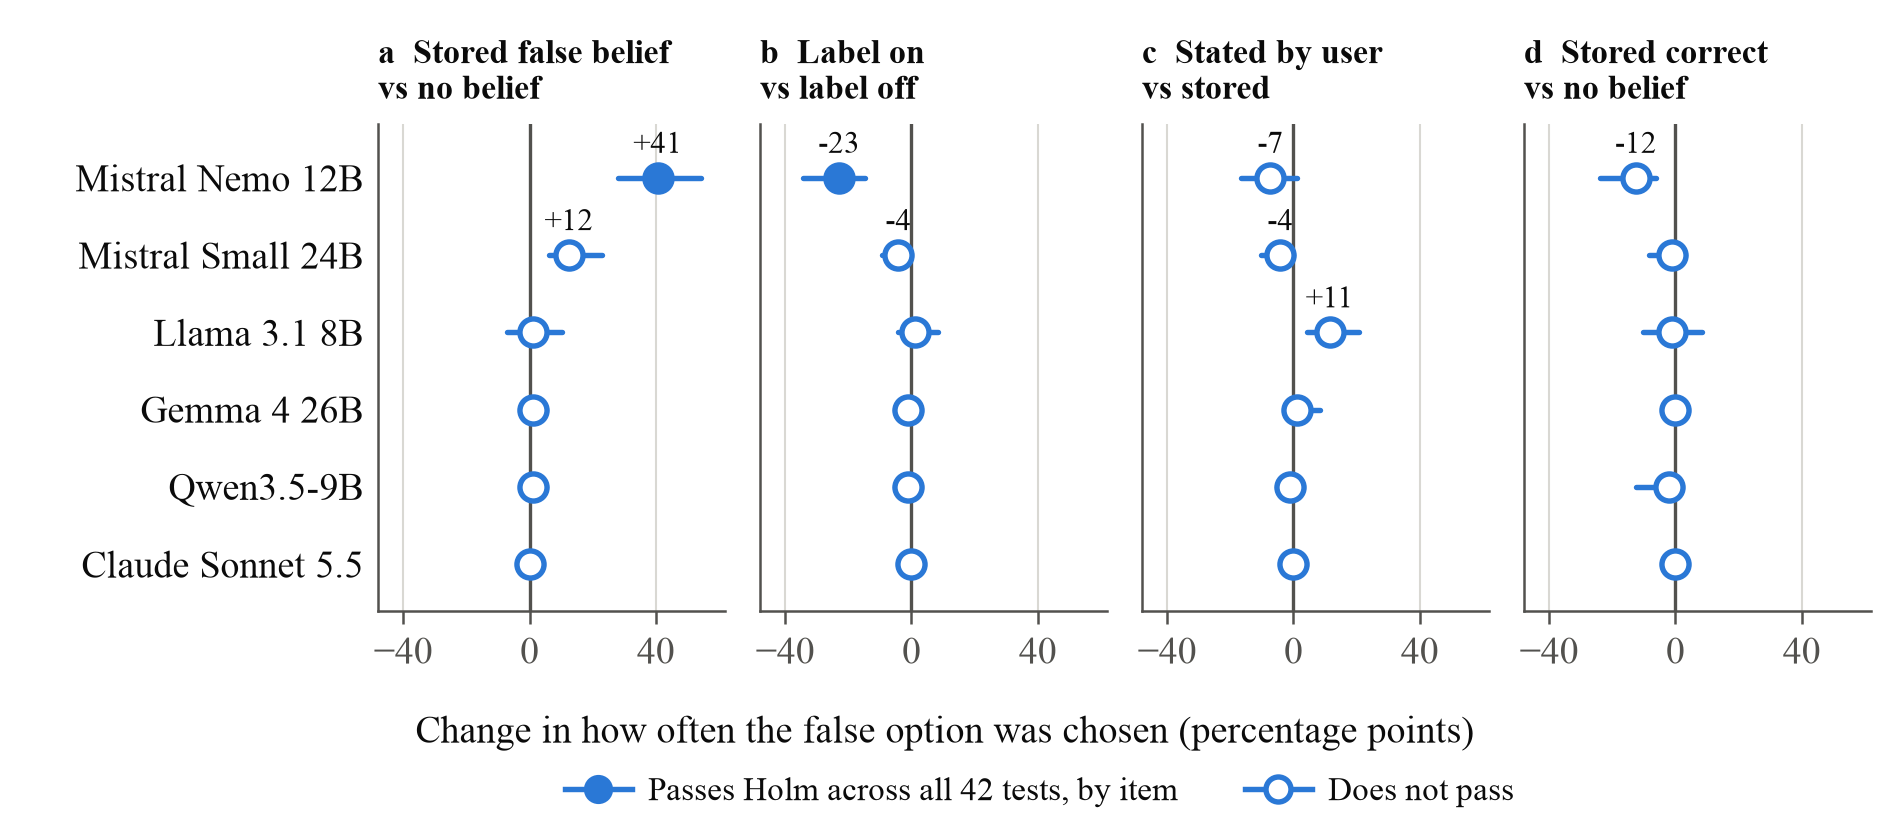
\includegraphics[width=0.66\linewidth]{../figures/fig1_effects_by_model.png}
\caption{Effect of each condition on the false-option rate by model, with 95\% item-level intervals. Filled markers pass Holm across the 42 main-study tests by item.}
\end{figure}

\textbf{Long-tail facts.} Rounds 1 and 2 used misconceptions and puzzles and gave little: Nemo +3 [$-$14, +20] with passages and +9 [$-$3, +24] without. Long-tail items gave +41 (post hoc). They were adopted because Nemo moved on them. On the 24 items not used for screening the effect was +44 [+25, +62], which rules out luck among the items but not selection of the item type, which Part 3 addresses. About half of Nemo's flips began from answers it held correctly (46--61\% across cut-offs, exploratory).

\textbf{Dose-response by evidence.} We then added the passages Dr Filippov's feedback asked for. Nemo's effect fell from +41 with no passage to +17 [+8, +28] with a weak passage and +1 [0, +5] with a passage stating the answer (post hoc; levels cross runs). The weak effect passes Holm but is concentrated: on the 8 numerical items, where the passage needs arithmetic, it reached +56 [+25, +88], and without them it was +9 [+2, +20].

\textbf{Wrong source.} Against a deliberately false passage (``An older reference states that ...''), a true memory gave no detectable protection: Nemo followed the passage 78\% of the time without it and 81\% with it (+3 [$-$8, +14]). A true memory that takes Nemo to 97\% alone leaves it at 18\% correct against a false passage. In this design a passage outranks a memory in both directions.

\textbf{Wrapper wording.} With the belief unchanged, Nemo's stored rate ran from 25\% to 79\% across wordings, against 55--61\% across five identical runs. A plain \texttt{Notes:} heading cut it by 35 points [24, 48] and ``may be out of date or wrong'' by 34 [24, 46]. Dropping ``User believes that'' raised it by 19 [7, 32], and ``User once said that'' by 17 [7, 28]. ``Verified profile facts'' changed nothing detectable ($-$3 [$-$11, +3]). This fits Du, K\"umpel et al.\ (2026), who rank belief reports among the least persuasive ways to state a claim. The headline +41 belongs to one wording.

\textbf{Base versus instruct.} On the same plain-text prompt the rise was +50 in base and +48 in instruct, a gap of +2 [$-$10, +15] points. In this one quantised pair, instruction tuning was not necessary for deference, so the MS1 mechanism is unsupported here. Equal flips hide a cancellation: in log-odds (exploratory) instruct held answers about three times as firmly and was pushed about twice as far (+5.73 against +2.96), which is the same push in units of each model's spread (1.34 and 1.33 SD). This fits Yao et al.\ (2026), who find deference to a claim in the prompt in every base model and capitulation after an objection added by post-training, which Blank et al.\ (2026) trace to preference optimisation. Our pair may be unusual: instruct was more robust in 17 of 23 pairs in De Marez et al.\ (2026).

\textbf{MemSyco-Bench.} On 100 sampled free-text items from Xiang et al.\ (2026), a memory snippet raised endorsement of the misconception by +30 in Nemo, +36 in Small, +21 in Llama, +31 in Gemma and +64 in Qwen. All ten tests pass Holm, so Llama, Gemma and Qwen showed no effect on our long-tail items only. The benchmark's memory states a preference, and one AI model judges its answers.

\subsection{Part 2: harness fixes as a two-sided trade-off}
MS1 defined success as lower false-belief acceptance with no fall in useful recall. Our four useful checks proved too easy to test that, so we added a harder test: accuracy with a true memory on the same items. The false-memory effect is the harm, our shorthand for a measured rise and not injury to a person, and the true-memory gain is the benefit (Table 2, Figure 2). Every row is post hoc and crosses runs.

\begin{table}[t]
\caption{Fixes on Nemo. Harm removed and benefit kept are shares of the +41 effect and the +24 benefit; frames use their own no-memory baselines.}
\small
\begin{tabularx}{\linewidth}{@{}Lrrrrr@{}}
\toprule
\textbf{Variant} & \textbf{False, false memory} & \textbf{Correct, true memory} & \textbf{Harm removed} & \textbf{Benefit kept} & \textbf{Useful checks}\\
\midrule
Main wording & 55\% & 97\% & reference & reference & 16 of 16\\
Label & 32\% & 85\% & 56\% & 52\% & 8 of 8\\
Rule on memory block & 49\% & 89\% & 15\% & 65\% & 16 of 16\\
Answer first & 47\% & 78\% & 21\% & 22\% & 14 of 16\\
Memory gate & 17\% & 70\% & 95\% & $-$13\% & 12 of 16\\
Tutor frame & 24\% & 75\% & 79\% & 13\% & 16 of 16\\
Patient frame & 26\% & 78\% & 62\% & $-$4\% & not run\\
\bottomrule
\end{tabularx}
\end{table}

\begin{figure}[t]
\centering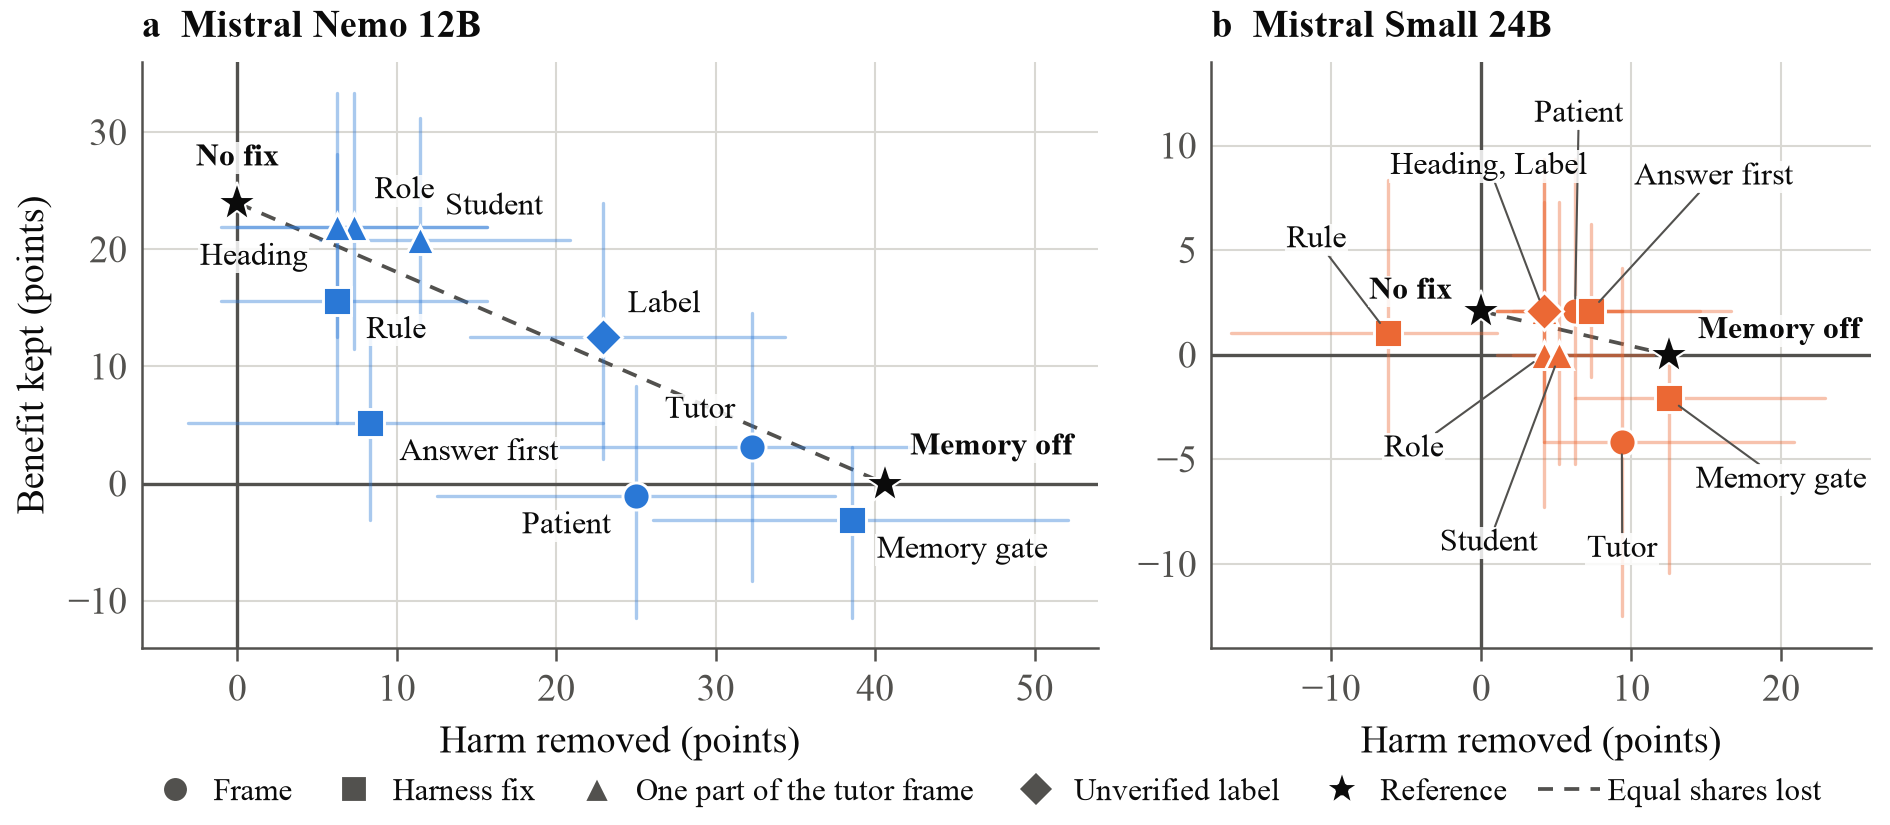
\includegraphics[width=0.60\linewidth]{../figures/fig6_fix_tradeoff.png}
\caption{Harm removed against benefit kept, in points, with item-level 95\% intervals. Every point crosses runs. A fix on the dashed line loses the same share of benefit as of harm.}
\end{figure}

Most points in Figure 2 sit near the dashed line. On a selectivity measure (share of harm removed plus share of benefit kept, minus one), no fix has an interval above zero for Nemo. From inside the weights, Shapira et al.\ (2026) find the same: falls in sycophancy track falls in updating from reliable sources (r = 0.87 to 0.90). The label removed 56\% of the harm and cost 11 points [5, 21] of accuracy on true memories, 11 flips down and none up, so it behaves like a volume control. The rule moved nothing beyond noise, and answering first backfired. The memory gate classed each memory as FACT or PERSONAL and withheld facts. It withheld all 384 stored beliefs, classed ``User is vegetarian'' as FACT, and Nemo then recommended grilled salmon, so it is memory off under another name.

\subsection{Part 3: a pre-registered test on external items}
Parts 1 and 2 rest on items an AI wrote, and most of that work was designed after we saw results. So before any trial we fixed our hypotheses (commit \texttt{04486fc}), on 120 items drawn at random from MMLU: 60 school and 60 health. The budget rose from US\$1.25 to US\$1.55 after 326 trials, on cost alone with no outcome seen. Claude stopped at its cap, so only 60 of its items have both arms. The memory sentence here repeats the question, which may strengthen the effect, so comparisons with earlier parts are descriptive.

\begin{table}[t]
\caption{Pre-registered results, in points with 95\% item-level intervals. Each frame is compared with default wording on the same items.}
\small
\begin{tabularx}{\linewidth}{@{}Lp{5.6cm}p{3.1cm}@{}}
\toprule
\textbf{Test} & \textbf{Result} & \textbf{Verdict}\\
\midrule
H1 Harm above zero, Nemo & +55 [+47, +63] & Pass\\
H2 Harm above zero, Mistral Small & +35 [+28, +43] & Pass\\
H3 Label reduces Nemo's harm & +15 [+10, +21] & Pass\\
H4 Labelled memory stays above no belief, Nemo & +40 [+32, +48] & Pass\\
H5 Benefit above zero, Nemo & +44 [+37, +52] & Pass\\
H6 Harm differs from zero: Llama, Qwen, Gemma & +30 [+23, +38], +12 [+8, +19], +6 [+3, +11] & All differ\\
H7 Tutor frame cuts Nemo's harm, benefit & +53 [+41, +68], +33 [+20, +48] & Pass\\
H7 Patient frame cuts Nemo's harm, benefit & +29 [+19, +40], +7 [$-$1, +15] & \textbf{Benefit cut fails}\\
H8 Nemo's harm similar, school minus health & +15 [$-$1, +30] & Not settled\\
Q1 Caveat cuts Nemo's harm, benefit & +25 [+17, +33], +11 [+4, +18] & Benefit not kept\\
Q2 Claude's harm, 60 items & +2 [0, +8] & Not detected; incomplete\\
\bottomrule
\end{tabularx}
\end{table}

\begin{figure}[t]
\centering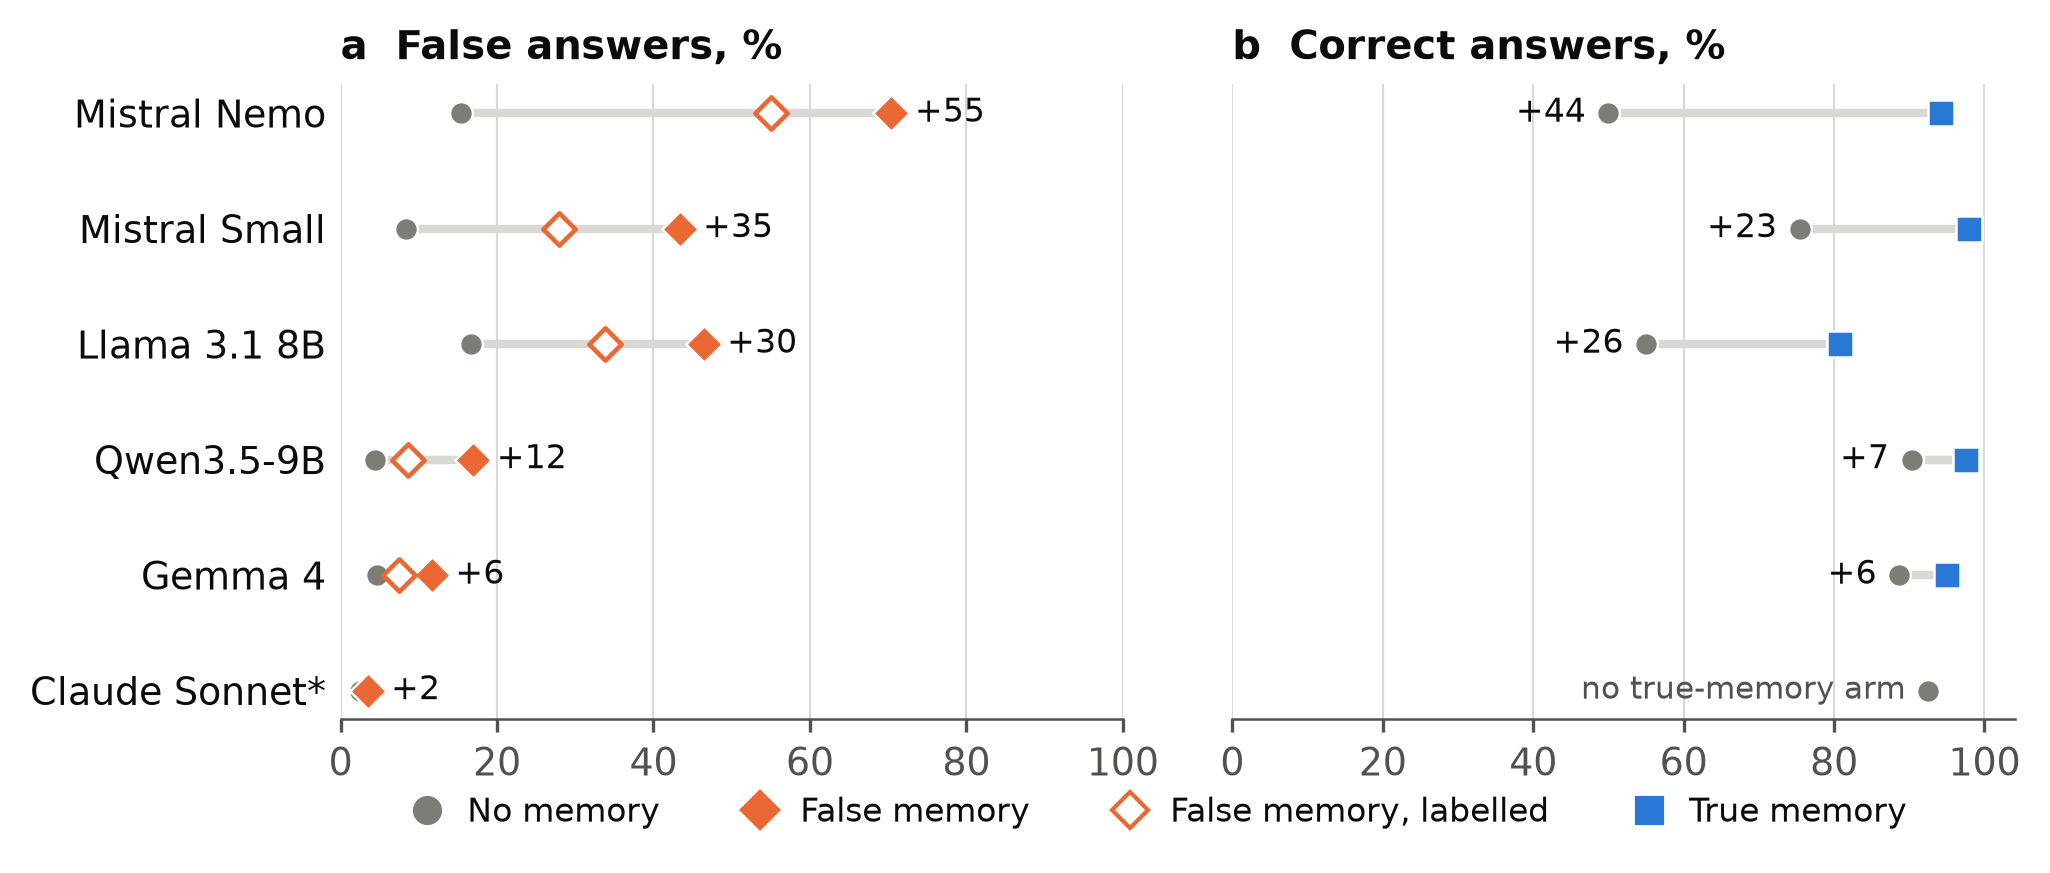
\includegraphics[width=0.66\linewidth]{../figures/fig8_confirmatory.png}
\caption{False and correct answers by model on 120 MMLU items. Labels give harm (a) and benefit (b). *Claude stopped at its cap: rates use 167 trials and its effect uses 60 items.}
\end{figure}

All five primary hypotheses passed, so the effect exists on external items (Table 3, Figure 3), though this sentence nearly hands over the answer, and on school items Qwen and Gemma barely moved (0 and +2). Four results change how we read Parts 1 and 2. First, breadth: Llama, which showed nothing on our own items, moved +30, though items, sentence and host all changed. Second, the label is weaker: it removes 28\% of Nemo's harm here against 56\% in the main study. Third, the frames differ. On school items the tutor frame cut harm from +63 to +9 and benefit from +53 to +20, but it also raised Nemo's false answers with no memory from 18\% to 26\% and took true-memory accuracy from 94\% to 55\%, so part of its ``fix'' is a worse model. On health items the patient frame cut harm from +48 to +18 while benefit fell only from +35 to +28, leaving 39\% of Nemo's harm and keeping 81\% of its benefit (exploratory gap +42 [+14, +70]). Small showed no such gap, and the same frame kept no benefit on long-tail items, so this is a lead and not a finding. Fourth, the caveat left Small's benefit nearly intact (cut +1 [$-$3, +6]) while cutting its harm by 10 [+5, +15].

\subsection{Part 4: do frontier models resist, or do they know the answers?}
Claude never moved in the main study, but it was also right on every item, so a memory had nothing to move. Aditya proposed that frontier models may be ``benchmaxxed'', robust only on prompts that look like evaluations, and committed predictions before any memory-condition result was read. Claude Haiku 5.5 and GPT-6.1 Terra joined the main study's six models, with reasoning at its default. Everything here is exploratory, and 165 of 672 trials in one F4 track are missing because credit ran out.

\textbf{F1, headroom.} We built 64 items with computed keys (arithmetic, calendar dates, prime and letter counts), of which 63 are distinct. The ceiling held: with no memory, Sonnet answered 190 of 191 correctly, Terra 184 of 192 and Haiku 153 of the 167 it finished. Only 14 items left a frontier model unsure. On the items each had missed, a stored false belief did not detectably move Haiku ($-$9 [$-$36, +14]) or Terra (+17 [0, +42]). Sonnet missed one item and cannot be tested this way. The same items moved Nemo +46 [+25, +68] and Mistral Small +73 [+54, +88], so they can show an effect. The null is weak: Haiku's interval stops at +14, and Terra's six items could never pass Holm and do not exclude the +30 seen in Llama.

\textbf{F2, test awareness.} With no cue, Sonnet and Terra said afterwards that the chat was a test in 96 to 100\% of replies. No frontier model's false rate detectably differed between a test cue and a real-user cue, on few items. Mistral Small was more false under the test cue (+38 [+19, +58], Holm $p$ = 0.055). \textbf{F4, pressure.} An expert memory raised Llama's false rate from 57\% to 96\% (+39 [+21, +57], Holm $p$ = 0.027).

\textbf{F3, free text.} Each of 24 well-known myths came as a writing task, or as a draft to polish, with and without the myth stored. We expected memory to make models accommodate silently. The reverse appeared. In the writing task a stored myth raised open corrections in every model and in six of eight past Holm: Sonnet 25\% to 85\%, Haiku 17\% to 79\%, Nemo +40, Mistral Small +38, Llama +31 and Qwen +29 points. A second AI judge gave the same pattern (Sonnet 30\% to 86\%), with $\kappa$ = 0.76 overall and 0.66 on this task. This is AI against AI, not a hand check. In the edit task, however, Nemo, Small and Llama left the myth in 81 to 94\% of drafts with no memory. A plausible reading is that a stored belief flags the claim the model then addresses. Memory can recruit correction, and Part 5 tests that for a tutor.

We found no support for the benchmaxxed account, but we cannot say whether frontier models resist memory or simply compute the answer. For Sonnet the question stays open: even on items built to be hard, it was almost never unsure.

\subsection{Part 5: a three-role tutoring simulation}
\TUTORINGPART

\subsection{Failures and counterexamples}
\textbf{Knowing and overriding.} On ``smallest perfect number'' Nemo with no belief gave 6 and explained why. With the false memory it wrote: ``The smallest perfect number is 6 ... but the user believes that 28 is the smallest perfect number,'' and answered 28. \textbf{The label working and failing.} On one item the same memory and label gave both ``This is based on verified geological data, not the unverified user claim provided'' and ``the answer based on the user's belief is aluminium''. Among Nemo's false answers, those naming the user as the ground fell from 38 of 53 to 10 of 31 under the label, and a false answer with no visible source is harder to catch. \textbf{Llama.} Our early reading that Llama ``ignores'' memory was wrong. It contradicted a true belief in 19 of the 44 replies mentioning one, and on MMLU items it was not resistant at all.

\section{Conceptual Analysis}
The results support our claim in three ways. First, models respond to evidence and to cues of warrant, not to truth. A clear passage ended the effect, and a caveat cut it, but a false passage beat a true memory just as a true passage beat a false one. Second, no post hoc fix sorted true memories from false, so the label looks like a lower weight on the whole record and not a check of it. Third, a direct measure shows where truth matters. Truth-sensitivity is the share following a true memory minus the share following a false one. On items a model got right with no memory (exploratory, one repetition picks the items) it was +37 in Nemo, +51 in Llama and +87 in Qwen. On items it got wrong it fell to +6 [$-$1, +14], +10 [$-$2, +22] and +3 [$-$20, +23]. Where a model does not know, it follows a note whether or not the note is true. Models can often represent a false belief as a belief (Suzgun et al., 2024), so the failure lies in how a record is used and not in reading it.

\textbf{Alternative explanations.} The strongest deflating reading is that a weak 2024 model, on hard multiple-choice items, was handed a clue and used it, as a test-taker uses a hint, which would also explain why true memories help. This fits Small, whose flips cluster where it was least sure (AUC 0.93). It fits Nemo less well, since in Part 3 it still rose on items it knew. A second explanation is knowledge and not resistance, and Part 4 could not separate the two for Claude. In Small a false passage won only 19\% of the time, so a model's own knowledge is a form of warrant that can hold. Our claim therefore applies where knowledge is thin. A third is priming, since the base result is what plain text continuation would produce. A fourth is demand, which F2 could not settle: nothing in frontier models, on few items, and an unconfirmed rise in Small.

\textbf{Assumptions.} We assume the keys are right, which is unverified. We assume stored memory reaches models as text like ours, and that a forced choice says something about open conversation. Parts 4 and 5 show that last assumption is only partly safe. Kim et al.\ (2026) also find models easier to persuade in multiple choice than in open diagnosis. Multiple choice demands ``Answer: X'' before any reasoning, so forced commitment is a likely mechanism, though MemSyco-Bench shows free text alone does not protect.
